\documentclass{article}
%\documentclass[a4paper,10pt]{article}
\usepackage{graphicx}
\usepackage{wrapfig}
\usepackage{lscape}
\usepackage{rotating}
\usepackage{epstopdf}
\usepackage{hyperref}
\usepackage[utf8]{inputenc}

% Default fixed font does not support bold face
\DeclareFixedFont{\ttb}{T1}{txtt}{bx}{n}{8} % for bold
\DeclareFixedFont{\ttm}{T1}{txtt}{m}{n}{8}  % for normal

% Custom colors
\usepackage{color}
\definecolor{deepblue}{rgb}{0,0,0.5}
\definecolor{deepred}{rgb}{0.6,0,0}
\definecolor{deepgreen}{rgb}{0,0.5,0}

\usepackage{listings}

% Python style for highlighting
\newcommand\pythonstyle{\lstset{
		language=Python,
		basicstyle=\ttm,
		otherkeywords={self},             % Add keywords here
		keywordstyle=\ttb\color{deepblue},
		emph={MyClass,__init__},          % Custom highlighting
		emphstyle=\ttb\color{deepred},    % Custom highlighting style
		stringstyle=\color{deepgreen},
		frame=tb,                         % Any extra options here
		showstringspaces=false            % 
		%fontsize=\small
}}


% Python environment
\lstnewenvironment{python}[1][]
{
	\pythonstyle
	\lstset{#1}
}
{}

% Python for external files
\newcommand\pythonexternal[2][]{{
		\pythonstyle
		\lstinputlisting[#1]{#2}}}

% Python for inline
\newcommand\pythoninline[1]{{\pythonstyle\lstinline!#1!}}



\begin{document}
	
\title{Routino: Users manual}
\author{Python code for doing batch travel time \& distance calculations}
%\author{Mike Allen (code). Kerry Pearn (user manual)}

\maketitle
\begin{flushleft}
\section{The functionality of the program}
Routino provides an open source solution for calculating travel time and distance between two locations.
Mike Allen created python code in order to make use of Routino to do batch calculations of many routes. This document describes how to use the python code and data files for your own batch calculations of travel times and distances.\\
\vspace{\baselineskip}
This document will describe these following files, in this file structure:


\begin{itemize}
	\item data\_etc
	\begin{itemize}
		\item profiles.xml
		\item uk\_postcodes.csv
		\item uk\_postcodes\_additional.csv
	\end{itemize} 
	\item output
	\begin{itemize}
		\item results.csv
		\item pivot\_results.py
		\item pivoted\_results\_distance\_km.csv
		\item pivoted\_results\_time\_min.csv
	\end{itemize} 
	\item batch\_process\_with\_running\_save.py
	\item from\_to.csv
	\item matrix.csv
	\item unstack\_matrix.py
	
\end{itemize} 

Figure \ref{fig:process_diagram} shows an overview of how the files listed above are linked together, and how the datafiles (blue) flow between the python code (yellow).

\begin{figure}[!h]
	\centering
	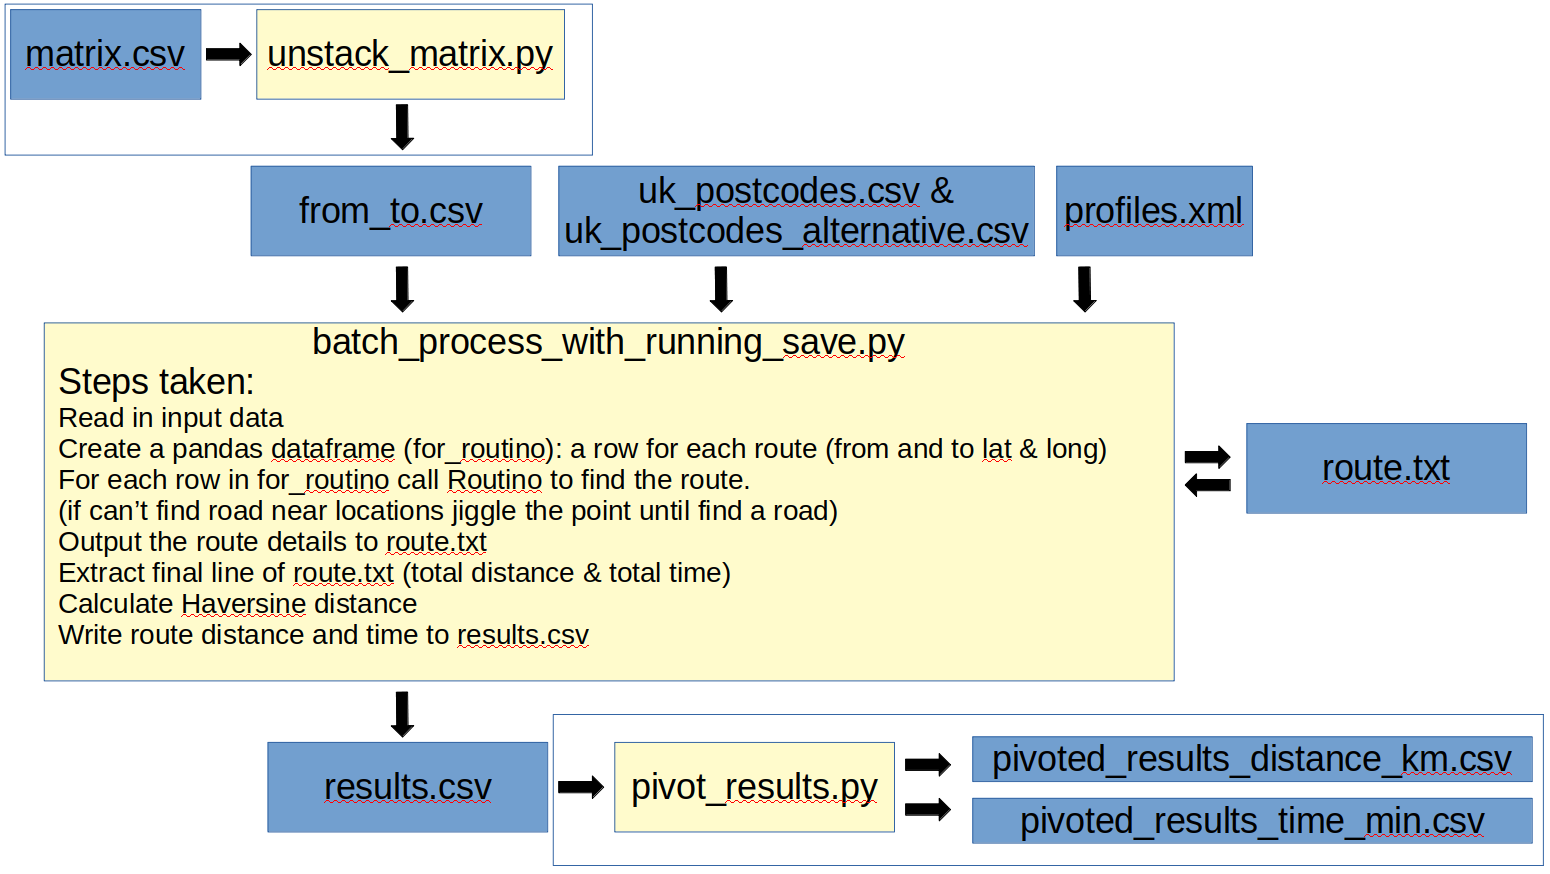
\includegraphics[width=1\textwidth]{images/process_diagram_1.png}
	\caption{A process diagram to represent the flow of information between files and Python code. Blue squares represent data files. Yellow squares represent Python code. Items in a boarder represent stages only required if you are working with a matrix (calculating a complete set of routes between a set of starting points and a set of ending points)}
	\label{fig:process_diagram}
\end{figure}


\newpage

\section{Describing the main program: batch\_process\_with\_running\_save.py}

The main Python code is \textit{batch\_process\_with\_running\_save.py}. This code does the core of the functionality - batch calculates the travel routes between multiple start and end points. This section will describe how it works and how to tailor it for your own purposes.

\subsection{The main part of this Python program}

The heart of the program is in the function \textit{get\_routino\_output}.
Here is the code (afterwards is a description of the functionality):

\newpage

%	"""Call Routino (pass start/end lat+long"""

\begin{python}
def get_routino_output(row):
  """Call Routino (pass start/end lat+long"""

  bashCommand = \	
  ('routino-router --dir=data_etc --trafig:process_diagramnsport=motorcar 
  --quickest --lon1=' + str(row['from_long']) + ' --lat1=' 
  + str(row['from_lat']) + ' --lon2=' + str(row['to_long'])
  + ' --lat2=' + str(row['to_lat']) + ' --language=en 
  --output-text --output-stdout >output/route.txt')

  os.system(bashCommand)
  last_line = extract_last_line('output/route.txt')
  time, distance, error = get_time_distance(last_line)
  haversine_distance = get_haversine_distance(
   					row['from_lat'], row['from_long'], 
					row['to_lat'], row['to_long'])
	return (time, distance, error, haversine_distance)
\end{python}

Routino is a separate programme that exists externally to this .py file. The .py file calls Routino using the line of code: "os.system(bashCommand)". This is essentially typing a command into the terminal.
The command is stored in the variable bashCommand. It is passing the necessary information the routino-router program.\\
\vspace{\baselineskip}
For the case above, the command is passing this information to routino:
\begin{enumerate}
	\item the data is stored in the subfolder data\_etc
	\item from the profiles.xml file use the values for motorcar
    \item find the quickest route
    \item for starting point use the values from the pandas dataframe row: from\_long and from\_lat
    \item for ending point use the values from the pandas dataframe row: to\_long and to\_lat	
    \item setting language to English
	\item send the output to the file output/route.txt
\end{enumerate}

Essentially we pass routino the start and end points (as lat and long values) and routino returns a text file (route.txt) that contains a step-by-step instruction of the routing information. Each row contains details of a section of the route, and the total route so far. Figure \ref{fig:route_txt} shows an example of this file.\\

\newpage

\begin{figure}[!h]
	\centering
	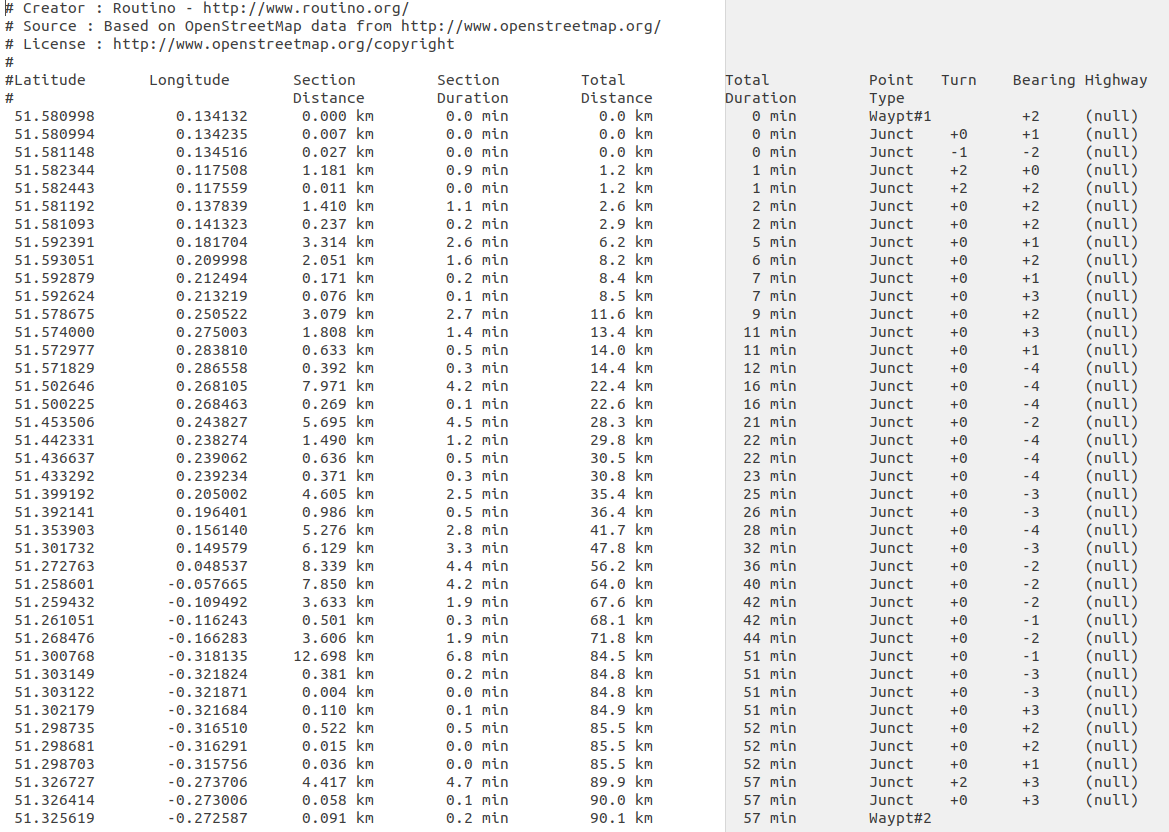
\includegraphics[width=1\textwidth]{images/route_txt.png}
	\caption{The contents of the \textit{route.txt} file}
	\label{fig:route_txt}
\end{figure}

As you can see, the final line of this file contains the total distance and time travelled for the whole route. For our purposes, we are only interested in this information. So for each route, we will extract this information from the final line of this file, write it to the output file, and then overwrite the contents of the route.txt file with the next journey. And repeat.\\

\vspace{\baselineskip}

One of the input files Routino uses is \textit{profiles.xml}. This contains the parameters for the transport selected via the command that was passed to routino. In our case this is \textit{motorcar}. Figure \ref{fig:motorcar} shows the associated properties for motorcar that routino will use to calculate the route:

\begin{figure}[!h]
	\centering
	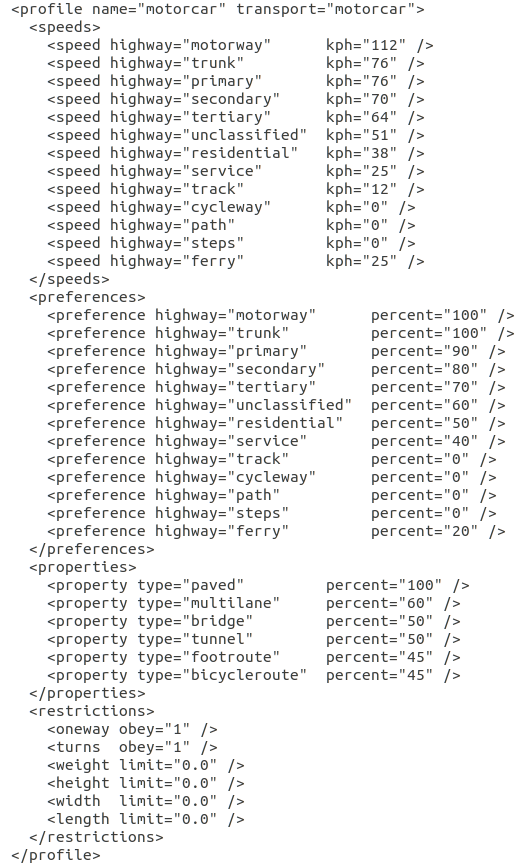
\includegraphics[width=0.5\textwidth]{images/motorcar.png}
	\caption{The motorcar properties contained in the \textit{profiles.xml} file}
	\label{fig:motorcar}
\end{figure}

\newpage

\subsection{How the code runs in sequence}

The program starts at this line of code:\\

\begin{python}
	if __name__ == '__main__':
\end{python}

Throughout the program the code prints it's progress. The first one of these is at the very start:\\

\begin{python}
	print(datetime.datetime.now().strftime("%H:%M:%S"), 'Start')
\end{python}

For cases in the program where a route can not be calculated by routino, the straight line distance between two points on the surface of a sphere is used (the haversine distance). This is then increased by a factor to take into account of the curvature of the roads (haversine\_tortuosity\_correction), and a constant speed of travel is used (assumed\_speed\_when\_imputing\_kph)\\

\begin{python}
	haversine_tortuosity_correction = 1.262
	assumed_speed_when_imputing_kph = 48.3
	correction_for_all_times = 1.000
\end{python}

As the program calculates each route, it writes the route result (along with any error catchers) to the output file as it goes along. Here we open the output file. 

\begin{python}
	output_filename = 'output/results.csv'
	results_header = ('from_postcode,to_postcode,from_lat,from_long,to_lat,' +
	'to_long,from_loc_identified,to_loc_identified,' +
	'route_locs_identified,time_min,distance_km,imputed,no_route\n')
	
	# Open output file
	with open(output_filename, 'w') as myfile:	
	myfile.write(results_header)
\end{python}

\textit{Note: To run multiple versions of Routino at once, make sure change the name of the two output files (results.csv and route.txt), otherwise will get errors as the route.txt will be written to and read by many programs, and so the values will be assigned to the wrong reference ID}.\\

\vspace{\baselineskip}

\subsection{Input files to edit to represent your case}
There are three files that you need to edit so that the program will run for your case.

\subsubsection{from\_to.csv}
This file contains all of the routes that Routino will calculate, one route per row. This input file needs to be a csv file with two columns. The first is the reference ID for the from location, and the second is the reference ID for the to location.

\begin{python}
    # Load data
	print(datetime.datetime.now().strftime("%H:%M:%S"), 'Loading data')
	from_to = load_from_to('from_to.csv')
\end{python}

\begin{flushleft}{\footnotesize Note:  If you are working with a travel matrix (calculating a complete set of routes between a set of starting points and a set of ending points) then there exists a separate .py file (\textit{unstack\_matrix.py}) which can help you to create the \textit{from\_to.csv} file. That .py file takes as an input all the starting locations, and all the ending locations, and creates the required input file for each pairwise combinations.}\end{flushleft}

\subsubsection{uk\_postcodes.csv (\& uk\_postcodes\_additional.csv)} 
There exists two further input files (\textit{data\_etc/ukpostcodes.csv} \& \\
\textit{data\_etc/ukpostcodes\_additional.csv}) that contain three columns. The first column is the reference ID for the location, the second is the corresponding latitude, and the third is the corresponding longitude. The function \textit{load\_postcode\_lat\_long()} joins these two csv files into a single pandas dataframe, removes any spaces in the reference ID and drops any duplicates.\\

\vspace{\baselineskip}

This pandas dataframe is used to look up the reference ID (that is contained in the \textit{from\_to.csv} file, and get it's latitude and longitude values. If your routes contain a reference ID that does not already exist in either of these files, you need to add a new ID together with it's latitude and longitude to the \textit{data\_etc/ukpostcodes\_additional.csv} file.\\

\vspace{\baselineskip}

This code was initially set up to calculate routes between two postcodes (hence the variables names call this location reference ID "postcodes"), but any unique ID can be used to reference a location so long as that unique ID exists in the lookup file along with it's corresponding latitude and longitude.\\

\begin{python}
	postcodes = load_postcode_lat_long()
\end{python}

\subsubsection{profile.xml} 
As previously mentioned, this file contains all of the parameters used for the different modes of transport (speed on road types, and preferences for road types).

\subsection{Preprocessing stage}
This step populates a pandas dataframe with the to-from locations represented as their lat-long values.
Done in function \textit{merge\_postcodes\_with\_lat\_long()}, and the resulting pandas dataframe is called \textit{for\_routino}.

\subsection{Find fastest route and output result to \textit{results.csv}}
For each row in the pandas dataframe \textit{for\_routino}, pass the latitude \& longitude values for both the start and end points to routino, and it will return the travel time, travel distance and haversine distance. It will also return an error flag to capture whether it was not possible to calculate the route.\\

\begin{python}
	# Call Routino	
	travel_time, distance, error, haversine_distance = 
						get_routino_output(row)
\end{python}

If no route was found (error flag return True), this could be due to no road being identified at the start or end locations.\\

\vspace{\baselineskip}

The code tries to deal with this by moving the start/end points a small amount to find a nearby road. These small location adjustments are stored in the list of lists called \textit{offsets}, and incrementally moves the point along each of the four cardinal directions (N, S, E and W). If a road is found (by making these small location adjustments) then calculate the route from that point.\\

\vspace{\baselineskip}

If no road was found after moving the locations, use the Haversine distance and report that the route is imputed.\\

\vspace{\baselineskip}

Write the result to the output file \textit{results.csv}. The values written to the output file are:
\begin{enumerate}
	\item \textbf{from\_postcode}: starting location as reference ID
	\item \textbf{to\_postcode}: ending location as reference ID
	\item \textbf{from\_lat}: latitude of the starting location
	\item \textbf{from\_long}: longitude of the starting location
	\item \textbf{to\_lat}: latitude of the ending location
	\item \textbf{to\_long}: longitude of the ending location
	\item \textbf{from\_loc\_identified}: if "1", then could not locate a road at the start location. Need to use haversine calculation
	\item \textbf{to\_loc\_identified}: if "1", then could not locate a road at the end location. Need to use haversine calculation
	\item \textbf{route\_locs\_identified}: Set to "1" if either of the previous two columns are "1". Need to use haversine calculation
	\item \textbf{time\_min}: the time taken for the route
	\item \textbf{distance\_km}: the distance of the route
	\item \textbf{imputed}: if "1", then no route found. Use straight line and adjust (Haversine)
	\item \textbf{no\_route}: if "1", use straight line and adjust (Haversine)
\end{enumerate}

\vspace{\baselineskip}

Then move on to the next row in the pandas dataframe \textit{for\_routino}, and calculate the route for the next set of to-from locations.\\

\vspace{\baselineskip}

At the end of the program, remove the route.txt file that was created by Routino.
 
\section{Formatting the output file}

The output file \textit{results.csv} has the values for a route per row.\\

\vspace{\baselineskip}

If your data represents a travel matrix (a complete set of routes from a set of starting locations and a set of end locations), then use \textit{pivot\_results.py} to put the output values back into a matrix format.
Two output files are produced: one for distance; one for time.

\begin{itemize}
	\item output
	\begin{itemize}
		\item time\_min\_pivoted\_results.csv
		\item distance\_km\_pivoted\_results.csv
	\end{itemize}
\end{itemize}


\section{Calibration}
It is advised that the values from Routino are calibrated against 50 of the routes as calculated by Google.\\

\vspace{\baselineskip}

Manually select 50 of your routes that cover the spread of the distances \& durations across all of the routes.\\

\vspace{\baselineskip}
\textit{Here I will talk about the route distances, but repeat this for both of the distance and durations}. 

\vspace{\baselineskip}
Calculate the correction factor for each of the 50 routes. Where the correction factor is calculated as:

\[ correction factor = Google\_distance / Routino\_distance \]

Calculate the median correction factor. 
\vspace{\baselineskip}

Also plot a scatter chart of the correction factor against the Routino distance. See Figure \ref{fig:correction_factor_graph} to demonstrate this.


\begin{figure}[!h]
	\centering
	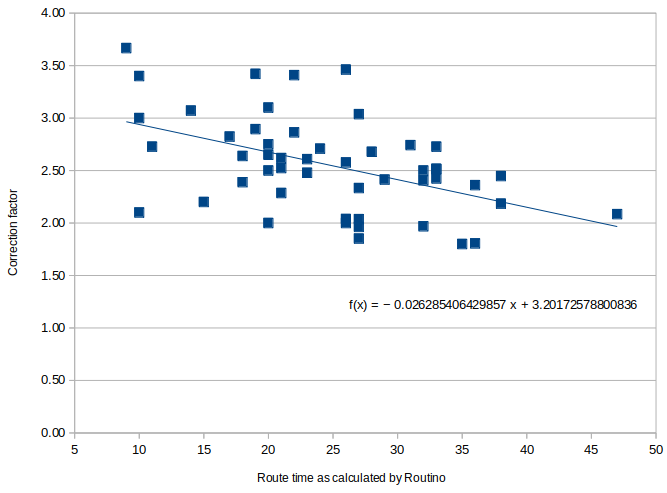
\includegraphics[width=0.8\textwidth]{images/correction_factor_graph.png}
	\caption{Plotting the correction factor against the Routino values}
	\label{fig:correction_factor_graph}
\end{figure}


\vspace{\baselineskip}

Decide whether it's reasonable to use the median of the correction factors for all, or whether there's a relationship such that the correction factor is dependant on the length of the route. 
\vspace{\baselineskip}

We have previously found that a constant value (the median) can be used for the correction factor for distance, but that the correction factor for time tends to be larger for the shorter routes, and so for those cases an equations (the trend line) is used. This can be linear, or a n order polynomial (as was the case for Scotland as the data showed an obvious kink/curve in the relationship).\\
\vspace{\baselineskip}
If the trendline in Figure \ref{fig:correction_factor_graph} is used, it will give a correction factor of 3.2017 when the route is of length 0, and for each unit increase in length, the correction factor will reduce by 0.026285.\\

\vspace{\baselineskip}

Ensure after these corrections that matrix (calculating a complete set of routes between a set of starting points and a set of ending points)the min value returned is 1.

\section{Using the travel matrix in a geographical modelling project}

Program: \textit{geographical\_modelling\_scenarios.py}\\

\vspace{\baselineskip}

If your routes form a travel matrix (where you have calculated a complete set of routes between a set of starting points and a set of ending points), then this section will describe how to use the program \textit{geographical\_modelling\_scenarios.py}, and the output file \textit{time\_min\_pivoted\_results.csv} (or \textit{distance\_km\_pivoted\_results.csv} - both from \textit{pivot\_results.py}) in order to model some geographical scenarios.

\vspace{\baselineskip}
The code treats all of the "from" locations as where a patient will begin their journey, and each of the "to" locations are where they can access a service.

The scenarios will explore the impact of having a different combination of these services open and receiving patients.

The code will create the full set of scenarios that will cover every possible combination of the services as "open".

\vspace{\baselineskip}

For each of the scenarios, the code will allocate each of the patient locations ("from") to the nearest open service ("to") location.

\subsection{Input files}

This program requires 2 input files. Here is the file structure this program requires:

\begin{itemize}
	\item data\_etc
	\begin{itemize}
		\item activity\_data.csv
	\end{itemize} 
	\item output
	\begin{itemize}
		\item pivoted\_results\_distance\_km.csv
		\item pivoted\_results\_time\_min.csv
		\item scenario\_results.csv
	\end{itemize} 
	\item geographical\_modelling\_scenarios.py
\end{itemize} 

\subsubsection{Input file: activity\_data.csv}

This is a csv file with two columns and a row per "from" location.
The "from\_postcode" contains the reference ID for the "from" location.
The "activity" column contains the number of patients that are at that location.
\vspace{\baselineskip}

The column titles must be kept as "from\_postcode" and "activity".
\vspace{\baselineskip}
This file provides the program with information about the number of patients at each of the "from" locations. The program will calculate weighted averages based on these activity values. If only one patient comes from each location, populate all of the values in column "activity" with 1.

\subsubsection{Input file: time\_min\_pivoted\_results.csv}

\textit{Change the code in the .py file to read in the equivalent distance file, if ever necessary}.

This is the output file from pivot\_results.py (which is the program that takes the Routino output as it's input file).

\subsection{Output files}

The program creates 1 output file: \textit{scenario\_results.csv}. It has a row per scenario.
The number of columns depends on the number of "to" locations there are.
\vspace{\baselineskip}

There are 4 columns to describe the full system:
\begin{itemize}
	\item \textbf{median\_travel}: median travel of all the patients in the whole system
	\item \textbf{max\_travel}: max travel of all the patients in the whole system
	\item \textbf{95pctl\_travel}: 95th percentile travel of all the patients in the whole system
	\item \textbf{activity\_within\_30}: total activity in the whole system within the threshold travel (in this case, it's 30 as shown in the column title)
\end{itemize}

\vspace{\baselineskip}

There is then a column per "to" location to show whether for that scenario it is open:
\begin{itemize}
	\item \textbf{location\_n}: whether the "to" location was open in the scenario (1 = open)
\end{itemize}

\vspace{\baselineskip}
And finally there are 6 columns per "to" location, to describe the group of patients that are in it's catchment (where n is the number of the "to" location). These 6 columns are:
\begin{itemize}
	\item \textbf{median\_n}: median travel for the patients that attended this "to" location
	\item \textbf{max\_n}: max travel for the patients that attended this "to" location
	\item \textbf{95pctl\_n}: 95th percentile travel for the patients that attended this "to" location
	\item \textbf{activity\_n}: the number of patients that attended this "to" location
	\item \textbf{activity\_within\_threshold\_n}: the number of patients that attended this "to" location within the threshold travel.
\end{itemize}

\section{Mapping}
Please consult the tutorial \url{https://youtu.be/QEZFnERpZxY} (YouTube channel HSMA: "Session 6B : An introduction to GeoPandas") to follow and apply GeoPandas to the results of this dataset.

\end{flushleft}


\end{document}
